\newpage
\chapter{Checking \texorpdfstring{\htmiss}{HTmiss} tails for data in the event display (11/07/2017)}
% The \texorpdfstring is so that bookmarks (in Adobe Reader, etc.) can be rendered properly. In the first {}, I specify the math symbols/special characters I want to use. In the second {}, I specify the normal text I want it to display in the bookmarks. Note, this doesn't affect my table of contents.

For pre-approval for SUS-16-038, I've been asked to look at the \htmiss\ tails in the event display at high \HT, LT, for data. I can use Fireworks (see~\ref{sec:fireworks}) as the event display visualiser. It's a case of identifying the excess events and inspecting them to see if there are any problems (reconstruction, etc.). By looking at the mountain range plot for the fully-unblinded 2016 data (the most current one is below), the bins containing "excess" events are indicated as those with large pulls (on the Pull axis, the units are in sigmas). So, to start with, I should be looking in the bins with a pull of 3$\sigma$ or more: $\njet = 3$, $n_{\mathrm{b-jet}} = 3$, $\HT > 600\GeV$; and $\njet \geq 6$, $n_{\mathrm{b-jet}} \geq 3$, $600 < \HT < 900\GeV$.

\begin{figure}[H]
\centering
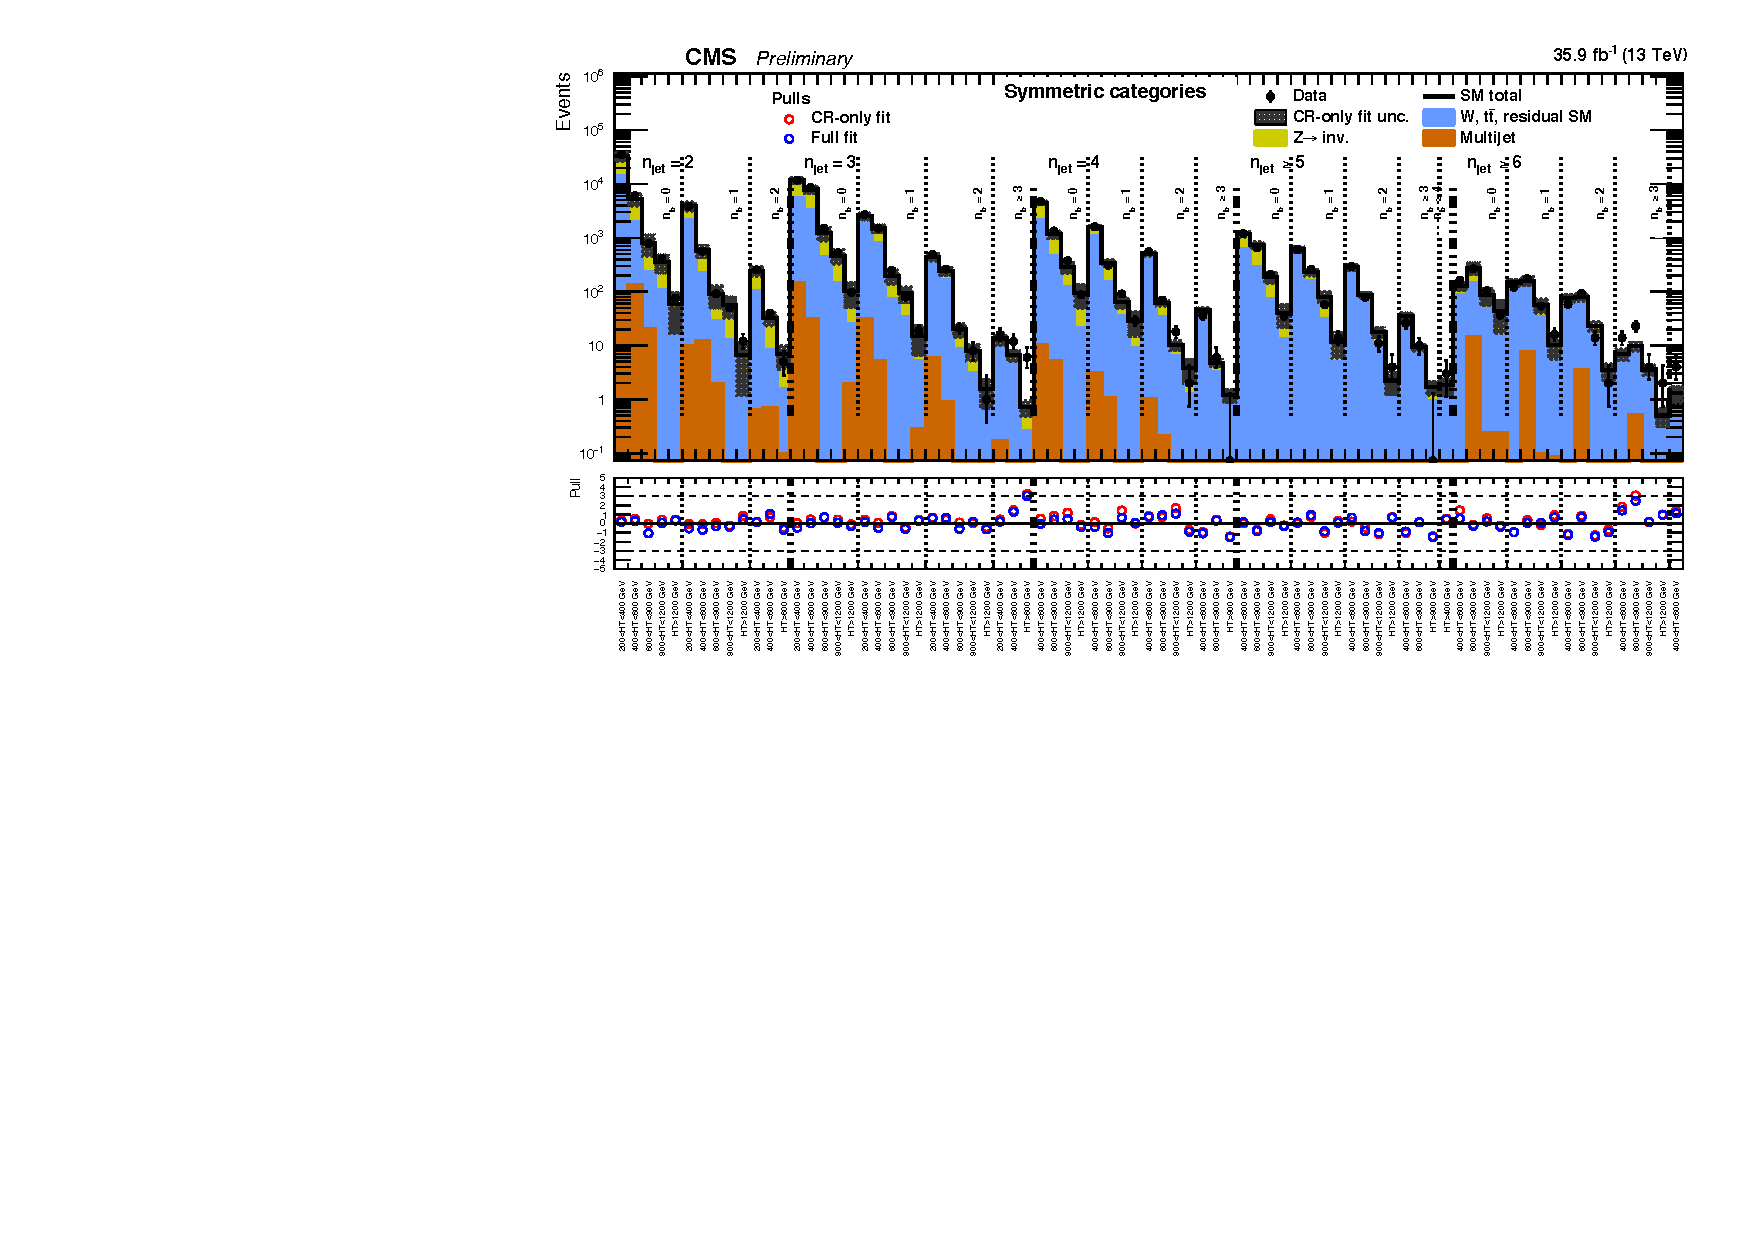
\includegraphics[width=\textwidth]{./sec27/summaryPlot_Symmetric_prefit_overlay_fit_b.pdf}
\caption{Mountain range plot showing the signal region events binned by (symmetric) \njet, $n_{\mathrm{b-jet}}$ and \HT with the fully unblinded 2016 data at 35.9 fb$^{-1}$. }
\end{figure}

% CAN REPLACE WITH FINAL MOUNTAIN RANGE PLOT ONCE IT'S IN PAPER, AND PAPER'S PUBLISHED

The above plot is taken from \url{http://www.hep.ph.ic.ac.uk/~klo2/RA1/BTagFormula/FullFit/Log/20170630/Unblinding36fb2017_v14_formulaSyst/postFitNorm/summaryPlot_Symmetric_prefit_overlay_fit_b.pdf}. I can apply cuts to select these bins and print out the run, lumi and event numbers. I can then use Lucien's script (\url{https://github.com/lucien1011/LittleFWLite/blob/master/SkimEDM/skimMiniAOD_EvtListAndPD_cfg.py}) to skim over the miniAOD, consolidate those events in a new root file, and then analyse them with Fireworks.

If I clone the repository (\url{https://github.com/lucien1011/LittleFWLite}, master branch) I can skim over the miniAOD, provided I supply the right input. The script \textbf{Utils/TextFileHandler.py} handles that. I need to add the run, lumi and event numbers (in that order) for each event to a text file, with one event per row. The config details the location of this text file. Because of the nature of the code, I need to clone at Imperial. I've forked it so I can do my own development and not mess up the original, so the command to clone it is

\begin{lstlisting}[belowskip=-0.7cm, language=sh, numbers=none]
git clone git@github.com:eshwen/LittleFWLite.git
\end{lstlisting}

As I'm using my own fork of the repo, I can push any changes to \texttt{origin master}.


\section{Retrieving the event information}

To get the event information, I can use AlphaTools at Imperial. On the v1.10.x branch, in \textbf{Analyzers/EventDisplay/}, there's a script called \textbf{Displayer\_HighNb\_cfg.py} which can create an RA1-style event display and a list of the events, after cuts, with their relevant information. I just needed to change the cuts to suit my needs, as well as the output file names and directory. It is already configured to run over 2016 data. I also had to edit L129 and L176 of \textbf{./Modules/Displayer.py}, changing \texttt{objTag = ""}. The leaf "pseudoJetFlag" is not in the newer trees, so I get errors if I leave those references in. Once I had made those changes, I could just run the script. The output folder contains text and pdf files for each data set that was run over. The text files contain the run number, lumi section and event number for each event that I need for the next step. The pdfs contain the RA1-style displays -- with one pdf per data set -- that show the event information, \alphat\ distributions, the properties and tracks of the hardest objects, and some calorimeter information.

The RA1 displays are quite helpful. Fireworks doesn't distinguish between regular jets and $b$-jets (and we need to know which is which). So I added some code in \textbf{Displayer.py} to change the colour of the $b$-jets in the circular plot and the square $\eta-\phi$ plot, as well as add a legend entry for them. But it turns out that the $b$-tag working points we were using were out of date. They are stored in a dict in \textbf{\$ALPHATOOLSDIR/Data/BTagWorkingPoints.py}, and the \texttt{outString} string in the \texttt{printJets} function of \textbf{Displayer.py} calls the values in this dict. The portion of the string \texttt{bCategory("CSV",jet.btagCSV)} appends L, M or T (whether it uses the loose, medium or tight working point) to the bit in quotes, and then pulls the corresponding value from the dict. So I just had to change it to \texttt{bCategory("CSVv2IVF",jet.btagCSV)}. Then I could add \texttt{if} statements in the jet loops of \textbf{Displayer.py} to \uline{draw the $b$-jets that satisfied the medium working point (\texttt{phyobj.btagCSV > 0.8484}) in dark red}.


\section{Skimming the miniAODs}

Now I can use LittleFWLite to skim over the miniAODs in the data set, and output the selected events into a new root file. If I go to the directory (\textbf{$\sim$/LittleFWLite/}), I need to \texttt{source setup.sh} and also do \texttt{cmsenv} in a recent CMSSW release -- I used 8.0.26 -- to source the main FWLite and FWCore modules.

\fcolorbox{Violet}{Dandelion}{\begin{minipage}{\textwidth}
If I go to the CMSSW GitHub repo (\url{https://github.com/cms-sw/cmssw}), there are lots of modules in different directories. If I follow the Flat Tree Production instructions, there's a line with \texttt{cat >> .git/info/sparse-checkout <<EOF}, and different modules below. I could add FWCore in that list of modules, then escape the list by typing \texttt{EOF}. Then I can continue with the instructions and compile, etc., so the modules I listed are included in the CMSSW directory I'm using. This is handy if I ever need specific CMSSW modules that aren't part of the standard workflow.
\end{minipage}}

In the script \textbf{SkimEDM/skimMiniAOD\_EvtListAndPD\_cfg.py}, I needed to make sure I passed \texttt{runAAA=True} to the \texttt{getFilesFromPD} function in the \textbf{Utils/DBHandler.py} script. To run over every miniAOD file in the data set, I could leave the \texttt{True} alone in \texttt{options.register('allFiles'}. However, this can take ages to run and isn't worth it unless I want to process a lot of events. So it's easier to just change it to \texttt{False}. This way, only files that contain the event information I supply are run over. Then I had to make sure the data set name , text file path, and output file path were correct. The syntax for the primary data set is quite specific. As the code uses the DAS to search for the data set and its files, it needs to be entered in the same format as a DAS query. I should look up the data set name on DAS by typing the process and run era, then using \verb!*!s for the rest of the query. I could then run the config with

\begin{lstlisting}[belowskip=-0.7cm, language=sh, numbers=none]
cmsRun skimMiniAOD_EvtListAndPD_cfg.py
\end{lstlisting}

I should get the log on-screen indicating the root files being opened and the events being processed.


\section{Using Fireworks to check the event displays}

Once I had the \ROOT file of the events I needed, I could use Fireworks to look at the event displays. For stand-alone tarballs, the commands to download and install it are different for the different versions (see~\ref{sec:fireworks}). However, it is fully integrated within CMSSW from CMSSW\_3\_X\_X. As I was using CMSSW\_8\_0\_26, I just needed to \texttt{cmsenv}, then I could run it with

\begin{lstlisting}[belowskip=-0.7cm, language=sh, numbers=none]
cmsShow <path to root file>
\end{lstlisting}

If on a remote server, I need to connect with \texttt{ssh -X} or \texttt{-Y} for X11 forwarding. I initially got some errors when trying to load the program, but entering the command \texttt{defaults write org.macosforge.xquartz.X11 enable\_iglx -bool true} into the terminal, locally, then restarting my Mac fixed the problem.

I can switch between events in a \ROOT file by pressing the big green arrows. I can add annotations to physics objects -- to show their properties -- by right-clicking over the object and pressing "Add Annotation". I can also drag the annotation to move it, and a grey line connects it to its object to avoid confusion with other, possibly similar objects. I can also save files, the main display being labelled a $\rho-\phi$ plot with File$\rightarrow$Export Main View Image.

I couldn't find any obvious anomalies in the event displays. There were several jets, as expexted, high \etmiss, and the occasional high-\pt muon. One of the annotated displays is below.

\begin{figure}[H]
\centering
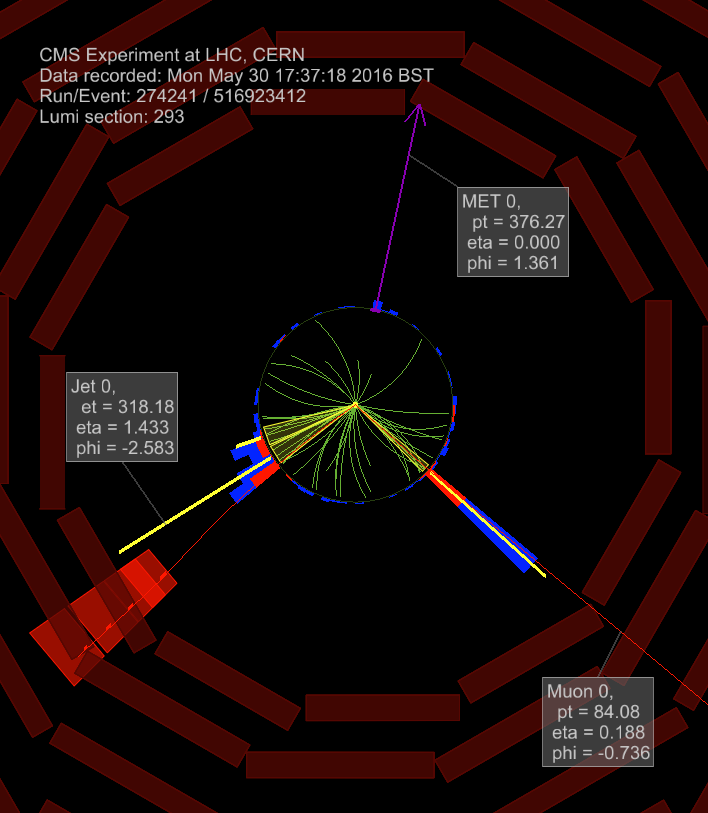
\includegraphics[width=120mm]{./sec27/skimHTMHT_Run2016B_3j_3b_ev1.png}
\caption{The event display from an "excess" event in the /HTMHT/Run2016B-03Feb2017\_ver2-v2/MINIAOD primary data set. The leading objects are annotated, as well as the event information.}
\end{figure}


\section{Conveying the results on Imperial's web pages}

Using some software developed by Ben and other IC people, I can use HTML and web-based languages to upload plots, etc., in a clean layout on Imperial's website. By logging onto lx00 or lx01, I need to do

\begin{lstlisting}[belowskip=-0.7cm, language=sh, numbers=none]
mkdir ~/public_html # Folder name must be this
mkdir -p CMS/RA1/AN-17-122/EventDisplays
cd CMS/RA1/AN-17-122/EventDisplays
git clone https://github.com/ic-coders-club/plotify.git
\end{lstlisting}

Then I will have a web page that I can view on a browser, of the form \textbf{www.hep.ph.ic.ac.uk/$\sim<$user$>$/$<$path below home dir minus "public\_html/"$>$}. From the above commands, it is \url{www.hep.ph.ic.ac.uk/~ebhal/CMS/RA1/AN-17-122/EventDisplays}. After this, I copied the Fireworks and RA1 event displays to \textbf{plotify/plots/}. The pdfs needed to be converted to png. To do this, I can just type

\begin{lstlisting}[belowskip=-0.7cm, language=sh, numbers=none]
for file in */*pdf; do convert -density 150 $file -trim ${file/pdf/png}; done
\end{lstlisting}

Next I had to add a \textbf{config.js} file, which contained code to point to the images to display, as well as how to organise and divide them up. Then I added an \textbf{index.html} file, which took care of the layout of the web page and the sub-headings, etc. The \textbf{style.css} file generated the colours and font. The link to all the event displays is at \url{http://www.hep.ph.ic.ac.uk/~ebhal/CMS/RA1/AN-17-122/EventDisplays/plotify/}. The Fireworks and RA1 displays are shown, with one event per page. As the Fireworks displays don't distinguish between regular and $b$-jets, I can match the circular plot in the RA1 display to the jets in Fireworks.

\section{Remaking the RA1 trees to include all muons in the event displays}

By default, in the RA1 display none of the muons aren't plotted; presumably because they fail at least one of the acc/ID/isolation/$\Delta R$ requirements. Because the code that produces the plots runs over the trees located at Imperial. The cuts that are applied during tree production means that none of these muons are actually stored in the trees. But with the skimmed miniAODs I have of the excess events, we should be able to reproduce the trees of those events, but leave in all the muons. Then I can run over these new, small trees in AlphaTools to produce RA1 displays that contain the muons and their properties.

Using Heppy/CMGTools in CMSSW, I needed to lower the thresholds for muons in \textbf{RA1/python/buildSequence.py}. Then add this snippet to L23 in \textbf{./analyzers/AtEventAttributesPrep.py} so all muons are included in the trees:

\begin{lstlisting}[belowskip=-0.7cm, language=python, numbers=none]
and e.relIso < 0.12 and e.miniRelIso < 0.2
\end{lstlisting}

This is due to the event selection and tree content, and full content are separate. So CMGTools needs to cut on right muons and save loose muons. I then needed to make a new function to skim over data locally in \textbf{RootTools/python/samples/ComponentCreator.py}, using the function \texttt{makeMCComponentFromLocal} as a template. I had to tweak it to omit MC-specific variables and include data-specific ones. The function looked like this:

\begin{lstlisting}[belowskip=-0.7cm, language=python, numbers=none]
def makeDataComponentFromLocal(self,name,dataset,path,pattern=".*root"):
    component = cfg.DataComponent(
        dataset=dataset,
        name = name,
        files = path+"/"+dataset+".root",
        triggers = [],
        intLumi = 1,
    )
    return component
\end{lstlisting}

Once that was done, I could make a components file containing the skimmed miniAODs, using \textbf{RA1/python/components/components\_Data\_2016.py} as a template. I had to replace the components with my own and change the line

\begin{lstlisting}[belowskip=-0.7cm, language=python, numbers=none]
components = [kreator.makeDataComponent(**s) for s in componentList]
\end{lstlisting}

to

\begin{lstlisting}[belowskip=-0.7cm, language=python, numbers=none]
components = [kreator.makeDataComponentFromLocal(**s) for s in componentList]
\end{lstlisting}

To match the input required for the function above, my components looked like this:

\begin{lstlisting}[belowskip=-0.7cm, language=python, numbers=none]
HTMHT_Run2016H_6j3b = dict(
    name = "HTMHT_Run2016H_6j3b",
    dataset = "skimHTMHT_Run2016H_6j_3b",
    path = "/home/hep/ebhal/EventDisplay_MHT_6j_3b/\ROOT_files",                                                                                                                                 
)
\end{lstlisting}

Finally, I edited the config file \textbf{RA1/cfg/run\_AtLogic\_Data\_cfg.py} to include my component file and my function to make the data components from local files. One problem I ran in to was that the config described my components as "data" (instead of MC). Normally, this requires a JSON associated with the data set. But if I just commented out \texttt{jsonAna} in the list \texttt{susyCoreSequence} in \textbf{TTHAnalysis/python/analyzers/susyCore\_modules\_cff.py}, I could bypass the JSON stuff as it's not needed in this case. Finally, I could run the config with

\begin{lstlisting}[belowskip=-0.7cm, language=sh, numbers=none]
heppy TEST_Skim run_AtLogic_Data_cfg.py
\end{lstlisting}

But when I looked at the trees, few muons were present. It seems some were still failing the selection/ID requirements. If I edited \textbf{RA1/python/treeContent/baseContent.py} and added the line

"inclusiveMuons" : NTupleCollection("allMuon", slimLeptonType, 50, help="All muons passing very loose selection conditions"),

around L223, some of these failing muons would be included in the trees. The rest can be added if I commented out L179-181 of \textbf{PhysicsTools/Heppy/python/analyzers/objects/LeptonAnalyzer.py}, which removes the selection criteria on these inclusive muons. I only need to leave the statement \texttt{mu.track().isNonnull()}. The leaf prefix would be "allMuon". So I could see their pT, eta, phi, etc. in the leaves "allMuon\_pt", and so on.

Once the trees were made, I had to ensure that AlphaTools ran over them. It's not as simple a process as I'd like. Firstly, I had to add the trees to \textbf{\$ALPHATOOLSDIR/Configuration/Samples/samples\_13TeV\_80X.py}. I could add each tree to the list that contained every sample, the syntax being

\begin{lstlisting}[belowskip=-0.7cm, language=python, numbers=none]
sampleList80X.addSample("HTMHT_Run2016B_3j3b", isData=True, parent="HTMHT")
\end{lstlisting}

Then I needed to add those samples to a "collection", like

\begin{lstlisting}[belowskip=-0.7cm, language=python, numbers=none]
sampleList80X.addCollection("EshsSkimmedExcessSamples",
                            ["<sample>",
        ])
\end{lstlisting}

I also needed to change the variable \texttt{basedirNominal} in \textbf{Configuration/config\_cfi\_2016\_skim.py} to point to the location of my trees. To include the "allMuon" objects (as they are different to regular muons), I had to add an entry for them in \textbf{Producers/Config/MakePhysObjects\_Setting.py} in the same format as the others. I also needed to add the \texttt{event.incMuon} entry to \textbf{Producers/MakePhysObjects.py} and add equivalent code to the event display scripts (\textbf{DefaultDrawSetting.py} and \textbf{Displayer.py}). Finally, I just needed to make sure my collection was referenced in \textbf{Analyzers/EventDisplay/Displayer\_HighNb\_cfg.py}. After looking at them, Rob concluded that we looked into the events in enough detail and that there were no obvious problems. The reply he gave to the conveners was "We have studied 29 events in the bins with the largest excesses (eq3j,eq3b) and (ge6j,eq3b) and find no anomalous behaviour."
